\documentclass{beamer}

\mode<presentation>
{
  \usetheme{Frankfurt}      % or try Darmstadt, Madrid, Warsaw, ...
  %% \usecolortheme{default} % or try albatross, beaver, crane, ...
  \usecolortheme[RGB={0,104,139}]{structure}%deepskyblue
  \usefonttheme{serif}  % or try serif, structurebold, ...
  \setbeamertemplate{navigation symbols}{}
  \setbeamertemplate{caption}[numbered]
  \useinnertheme{rounded}
}

\usepackage{array}
\usepackage{graphicx}
\usepackage{hyperref}
\usepackage{pxfonts}
\usepackage[english]{babel}
\usepackage[utf8x]{inputenc}

\usepackage{amsmath}
\usepackage{tikz}
\usetikzlibrary{arrows,shapes}
\setbeamercovered{transparent}
%% 
\title[Sandhi
\insertframenumber/\inserttotalframenumber]{Sandhi\\ Open Source Visual Programming Software}
\author[Sandhi Team, IIT Bombay]{Ambikeshwar Srivastava \\FOSSEE, IIT Bombay \\Manoj Gudi\\ CTO, Focus Analytics}
\date{August 22,2015}
\usepackage{beamerthemesplit}
\usepackage{beamerthemeshadow}
\logo{
\includegraphics[width=1cm height=2cm]{fosseelogo.png}
    \hspace{\dimexpr \paperwidth-2cm-5pt}

\includegraphics[height=1cm]{iitblogo.pdf}}

\begin{document}
\begin{frame}
\titlepage
\end{frame}

\begin{frame}
	\frametitle{Introduction}
	\begin{itemize}
		\item Sandhi is a visual programming editor based on GNU Radio
		\item Basic data structure in sandhi is the flowgraph
		\item It has been named Sandhi as it means connecting and conveys our idea of connecting various blocks to come up with a robust visual program
		\item Sandhi is aimed to become a visual programming tool for replacing LabVIEW
	\end{itemize}
\end{frame}

\begin{frame}
        \frametitle{Flowgraph}
        \begin{itemize}
        \item Flowgraph represents the connections of the blocks through which a continuous stream of samples flows
        \item The concept of a flowgraph is an acyclic directional graph with one or more source blocks (to insert samples into the flowgraph), one or more sink blocks (to terminate or export samples from the flowgraph), and any functional blocks in between.
        \end{itemize}
	\vspace{-0.14in}
        \begin{figure}
        \centering
        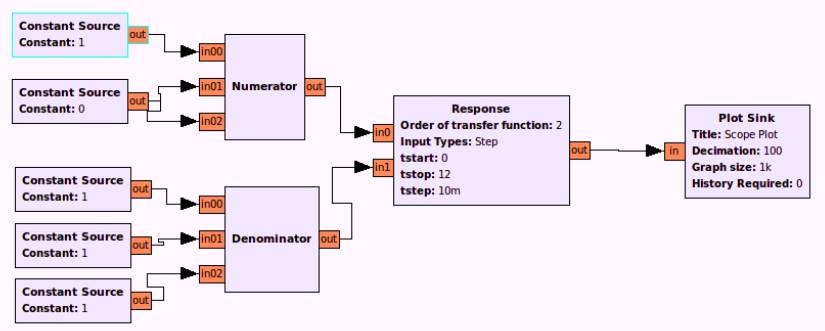
\includegraphics[height=2.8cm, width=10cm]{step_resp.png}
        \end{figure}
        \vspace{-0.2in}

\end{frame}

\begin{frame}
        \frametitle{Motivation to develop Sandhi}
        \begin{itemize}
		\item  Lack of proper open source alternative to LabVIEW.
		\item  Expensive proprietary software.
		\item  Being FOSS, it gives you freedom to modify, share and sell your application without any permission. 
        \end{itemize}
\end{frame}

\begin{frame}
        \frametitle{Development of Sandhi}
        \begin{itemize}
                \item GNU Radio
                \item sciscipy
                \item GRAS
        \end{itemize}
\end{frame}

\begin{frame}
        \frametitle{GNU Radio}
        \begin{itemize}
		\item GNU Radio is a free and open-source software development toolkit that provides signal processing blocks to implement software radios.
		\item Supposed to be used by the Electrical Engineering community for the purpose of digital signal processing 
		\item It has a rich module of implemented device drivers and thereby supports a range of devices
        \end{itemize}
\end{frame}

\begin{frame}
        \frametitle{Why GNU Radio?}
        \begin{itemize}
                \item GNURadio is a very promising visual programming tool as:
        \begin{itemize}
                \item it make very easy for the developer to abstract his code
                \item provides a very easy to use framework to the developer
                \item it is open source
        \end{itemize}
        \end{itemize}
\end{frame}

\begin{frame}
	\frametitle{sciscipy}
	\begin{itemize}
		\item Sciscipy is an Application Programming Interface 
		\item Aimed for Inter Process Communication with scilab when in workspace of Python programming language
	\end{itemize}
\end{frame}

\begin{frame}
        \frametitle{GRAS}
        \begin{itemize}
		\item GRAS stands for GNU Radio Advanced Scheduler
		\item It was impossible to implement the feedback with GNU Radio, which uses stock application schedular 
\textbf{Note:} Application Scheduler is responsible for threading, controlling the data flow and managing the use of the computer resources like processor time to various processes.
        \end{itemize}
\end{frame}

\begin{frame}
        \frametitle{Block in sandhi}
        \begin{itemize}
	\item Blocks are the basic building component of flowgraph
	\item Blocks have the property written in C++ or Python
        \end{itemize}
\end{frame}

\begin{frame}
        \frametitle{How to create a block}
        \begin{itemize}
        \item One can create a customized block with knowledge of C++ or Python
        \item Block developer have access to any library available in Python
	\item There are two files needed to create a block in sandhi:
		\begin{itemize}
			\item Functionality written in C++ or Python
			\item Properties written in xml file
		\end{itemize}
        \end{itemize}
\end{frame}

\begin{frame}
\frametitle{Work Flow}
\vspace{-0.14in}
\begin{figure}
\centering
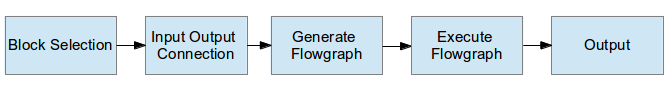
\includegraphics[height=2.8cm, width=10cm]{sandhi_presentation.png}
\end{figure}
\vspace{-0.2in}
\begin{itemize}
\item \textbf{Block:} A functional processing unit with inputs and outputs.
\item \textbf{port:} A single input or output of a block.
\item \textbf{Source:} A producer of data.
\item \textbf{Sink:} A consumer of data.
\item \textbf{Connection:} A flow of data from output port to input port.
\item \textbf{Flow graph:} A collection of blocks and connections.
\end{itemize}


\end{frame}\begin{frame}
        \frametitle{Experiments on sandhi: Data Aquisition}
        \begin{itemize}
	\item Single Board Heater System(SBHS) can controlled using sandhi
	\item Using Python serial library, one can set the fan,heat value to SBHS and receive temperature value from SBHS
        \end{itemize}

%  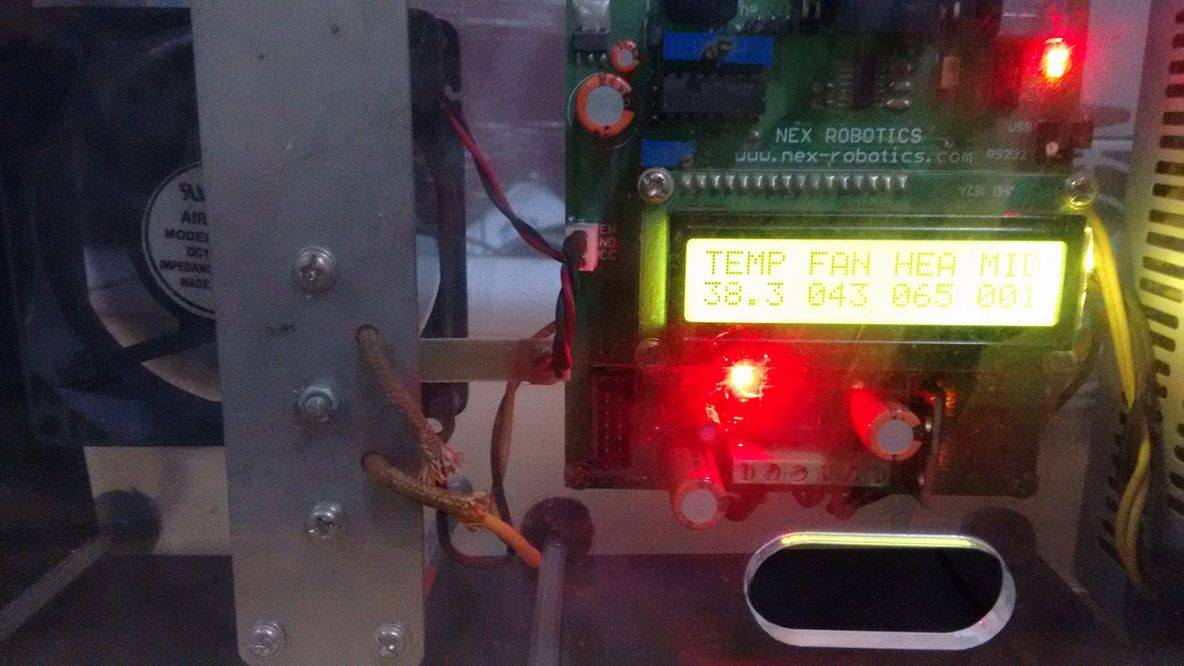
\includegraphics[width=.5\linewidth]{sbhs.jpg}
%  \caption{SBHS showing value of fan, heat and temperature}
%  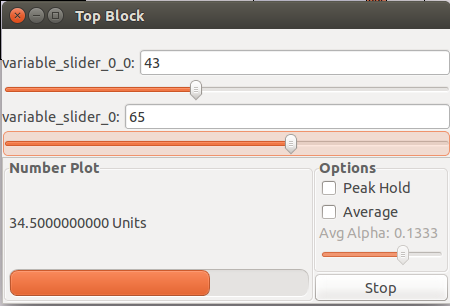
\includegraphics[width=.5\linewidth]{sbhs_img.png}
%  \caption{Output window with slider}
%\begin{figure}
%\subfigure[SBHS showing value of fan, heat and temperature]{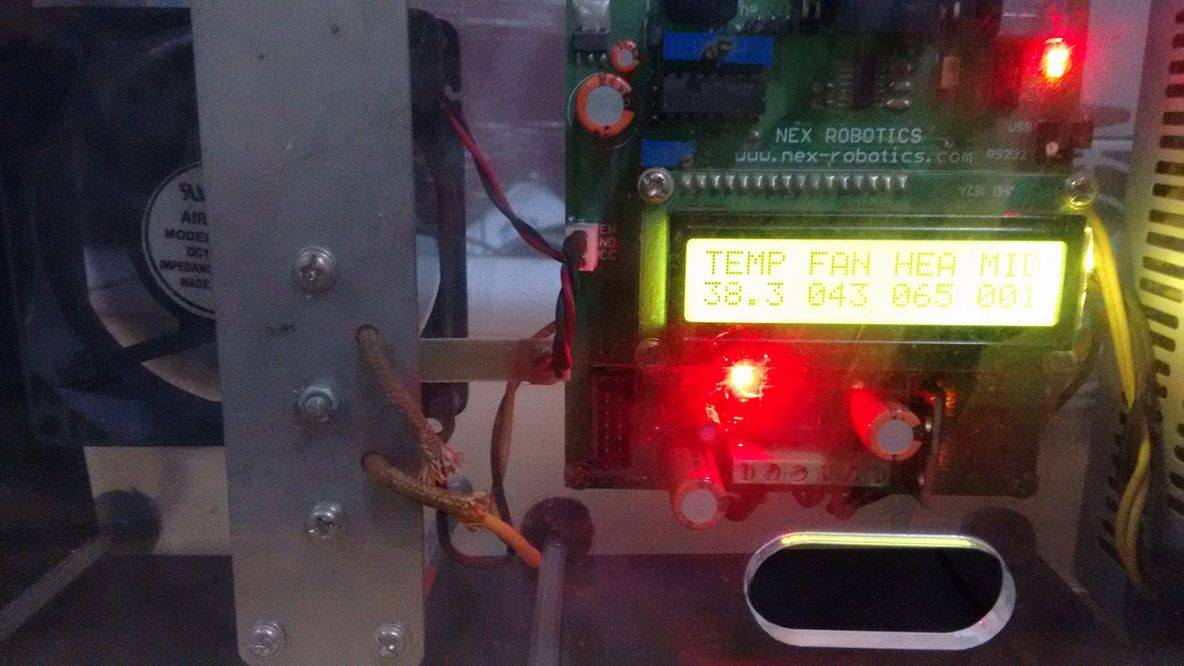
\includegraphics[width=5cm]{sbhs.jpg}}
%\subfigure[Output window with slider]{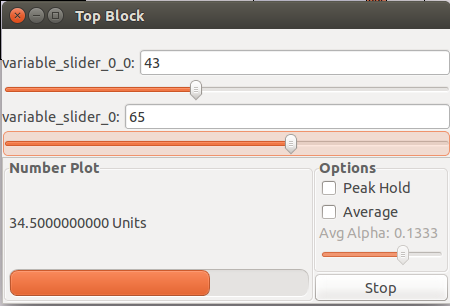
\includegraphics[width=5cm]{sbhs_img.png}}
%\caption{Single Board Heater system running on sandhi}
%\end{figure}
\end{frame}


\begin{frame}
        \frametitle{Experiments on sandhi: step response of transfer function}
        \begin{itemize}
	\item To perform step response the flowgraph is created as follows
	\item Flowgraph uses Numerator, Denomenator, Response and plot-sink block
	\item These blocks has been written in Python and response of system is calculated in scilab using sciscipy
        \end{itemize}
\end{frame}

\end{document}
